\documentclass{book}
\usepackage{graphicx, geometry, xcolor, fancyvrb, hyperref, ulem, microtype}
\graphicspath{ {./img/} }
\geometry{a5paper, left=20mm, right=20mm, top=10mm}
\begin{document}
\pagenumbering{arabic}
\pagestyle{plain}

\begin{center}
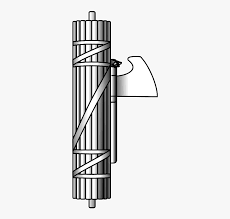
\includegraphics[width=3cm]{images.png}
\end{center}

\begin{flushleft}
\textbf{You say we live in a throw-away economy, what do you mean
    by that?}\\
Utility and satisfaction
No. And we will never have that word attributed to our cause.
Our stance on repatriation is that it is a cruel exodus
that divides but does not solve.
\end{flushleft}
\begin{flushright}

\textbf{What are some consequences of the throw-away economy?}
The consequences are innumerable; to list just 5 would be exhaustive
as each have their own ripple effect.
Planned obsolescence; those complicit in this, are usually not the higher-ups

\end{notation}

There is no such thing as a clothing shortage, yet because of convenience.
The quality of clothing has stagnated.
Two worlds that do not overlap.

Quality craftsmanship especially Britian's bespoke market, is too often overlooked. Consumers are brainwashed for inflated clothes, often produced in sweatshops or
in foreign countries.

If this is to be seen as a threat to morals and Christian values, then the party has nothing to comment on the matter. The state is bias from all Holy Books. In private, people will be allowed to love as they please and identify in which they choose. In public we ask, that children remain free to pursuit a nurturing and free childhood, in which they are not hammered down with sexuality and identification.

The way they're all so happy to throw eachother under the bus and go at eachother's throats just to chase power  is disgusting. They're literally the worst of u
\end{flushright}

\begin{flushleft}
    \textbf{Why do you strongly endorse domestic production?}
    Our productivity is at an all-time low.

\end{flushleft}

\end{document}
